\documentclass[11pt,border=4pt]{standalone}
\usepackage{amsmath,amssymb,bm,mathtools}
\usepackage[fontset=fandol]{ctex}
\usepackage{tikz}
\usetikzlibrary{arrows.meta,calc,patterns,angles,quotes,decorations.markings,decorations.pathmorphing}
\newcommand{\dd}{\mathop{}\!\mathrm d}
\newcommand{\e}{\mathrm e}
\tikzset{axis/.style={->,>=Stealth,line width=.45pt},world/.style={line width=.8pt},flow/.style={->,>=Stealth,line width=.7pt},ray/.style={->,>=Stealth,line width=.7pt},guide/.style={dashed,line width=.35pt},aux/.style={dashed,line width=.35pt},dim/.style={<->,>=Stealth,line width=.35pt},every node/.style={font=\small},force/.style={->,>=Stealth,very thick},gas/.style={fill=blue!7}}
\begin{document}
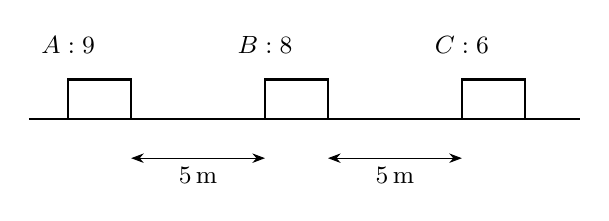
\begin{tikzpicture}\draw[world](0,0)--(7,0);\foreach \x/\s/\v in {.5/A/9,3/B/8,5.5/C/6}{\draw[world](\x,0)rectangle({\x+.8},.5);\node[above]at(\x,.7){$\s:\v$};}\draw[dim](1.3,-.5)--(3,-.5)node[midway,below]{$5\,\mathrm m$};\draw[dim](3.8,-.5)--(5.5,-.5)node[midway,below]{$5\,\mathrm m$};\end{tikzpicture}
\end{document}
